\section{Dispositif: Temps de vie du muon}

Cette manipulation a pour but la mesure du temps de vie du muon, en utilisant
les muons produits dans les rayons cosmiques. L'exp\'erience ne mesure pas la
charge des particules; on ne peut donc pas diff\'erencier les muons et
leur anti-particule avec le dispositif propos\'e.

Le dispositif (voir figure~\ref{fig:TpsVieMuon_disp}) est compos\'e de 4 grands ($\sim$ 1m$^2$) scintillateurs (voir section
\ref{subsec:scint}) coupl\'es \`a un (parfois deux) photomultiplicateurs (voir section \ref{subsec:PMT}).

\begin{figure}[!h]
    \centering
	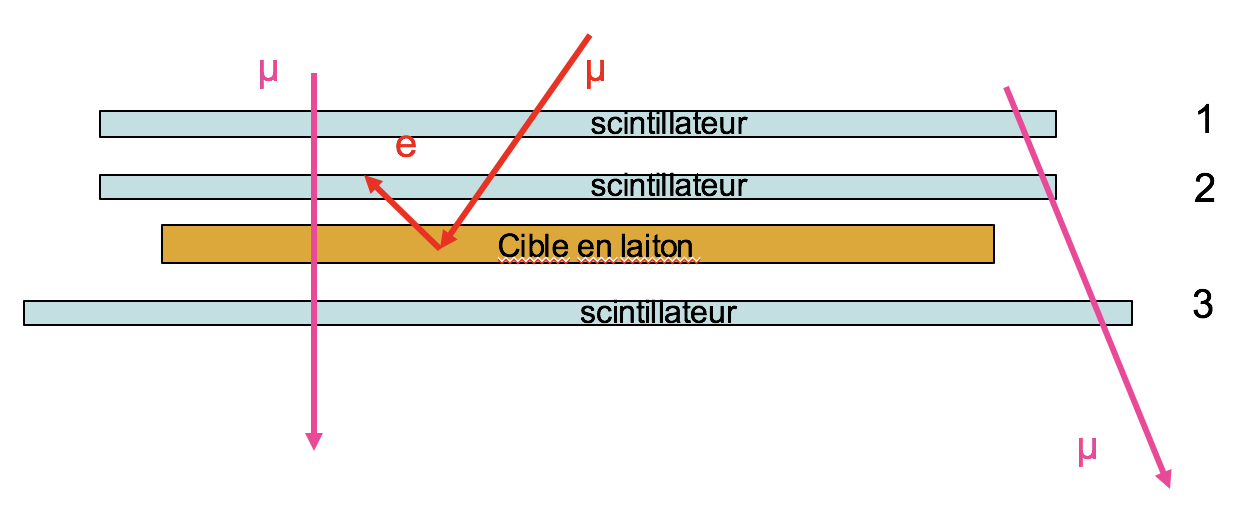
\includegraphics[width=\textwidth]{figures/Schema-Tps-de-vie.png}
    \caption{Schema du dispositif pour la mesure du temps de vie du muon.}
    \label{fig:TpsVieMuon_disp} 
\end{figure}

Le temps de vie \'etant mesur\'e pour des muons au repos, les scintillateurs sont plac\'es de part et d'autre d'une cible en laiton.
Une fois au repos, le muon se d\'esint\'egrera (avec une probabilit\'e de 98$\%$) en un
\'electron avec l'\'emission de deux neutrinos, selon la r\'eaction
$\mu^+ \rightarrow e^+ \nu_e \bar{\nu_{\mu}}$, avec un temps de vie moyen de 2.2 $\mu$s.
Vous allez donc mesurer pour chaque muon qui s'arr\^ete dans la cible le temps
entre la d\'etection de l'arr\^et du muon dans la cible et la d\'etection de
l'\'emission de l'\'electron (notre dispositif est incapable de d\'etecter
les neutrinos).

Le temps de d\'esint\'egration sera mesur\'e \`a l'aide d'un TDC (voir section \ref{sec:materiel}).
Le TDC ne fonctionne qu'avec des signaux digitaux répondant au standard NIM;
il vous faudra donc cr\'eer de tels signaux \`a  partir des signaux analogiques
qui sortent des photomultiplicateurs. Les signaux des photomultiplicateurs seront convertis en signaux NIM grâce à des discriminateurs. Avec ces signaux vous
pourrez concevoir une logique dite de declenchement (trigger) pour enregistrer
le temps de d\'esint\'egration sur le PC d'acquisition et pour ne pas
enregistrer n'importe quel temps entre deux signaux consécutifs qui pourraient
\^etre dus \`a du bruit \'electronique ou \`a des particules ne s'arr\^etant pas dans la cible.

Avant de concevoir cette logique de déclenchement de l'acquisition et de l'enregistrement des donn\'ees vous devrez effectuer une s\'erie de v\'erifications
et de calibrations pour vous assurer que les donn\'ees qui seront enregistrées
ont du sens:

\begin{center}
\fbox{
\begin{minipage}{0.75\textwidth}
\textbf{Les grandes étapes de la partie instrumentale :} 
\begin{quote}
  \begin{itemize}
    \item V\'erifier les signaux de tous vos PMs
\item étudier l'efficacité des PMs et mesurer le bruit de fond
\item calibrer le TDC
\item développer la logique d'acquisition de données
\item tester la logique avant de lancer l'acquisition pour la nuit
\end{itemize}
\end{quote}
\end{minipage}
}
\end{center}

\subsection{Agenda du laboratoire}
\begin{tabular}{p{0.2\linewidth} p{0.8\linewidth}}
Lundi & - Familiarisation avec le matériel\newline
		- Vérification des signaux analogiques des PMs à l'oscilloscope\newline
		- Mise en temps des signaux\newline
		- Mesure de l'efficacité d’un PM au choix en fonction de la tension et du seuil\\
Mardi & - Calibration du TDC et \textit{dual-timer}\newline
		- Développement et test de la logique simplifié\\
Mercredi & - Développement de la logique finale et prise de donnée \\
Jeudi et Vendredi & - Développement d'une simulation Monte-Carlo\newline
		- Développement du programme d'analyse\newline
		- Préparation de la présentation\\
\end{tabular} 

\subsection{Vérification du dispositif}
\textbf{Avec l'aide d'un assistant} régler les tensions des PMs de manière à 
avoir des signaux observables \`a l'oscilloscope. Les tensions de fonctionnement des PM du dispositif dit ``vieux'' et qui possède 8 PMs sont de l'ordre de 2000 à 2200V. \textbf{Ne dépassez en aucun cas 2200V sur ce dispositif}.

Une fois que vous avez identifi\'e les signaux des PMs à l'oscilloscope, observez-les et prenez note de leurs caract\'eristiques (amplitude, temps de 
mont\'ee, dur\'ee, etc.).

Vérifier qu'ils sont en temps. En effet pour pouvoir identifier un muon ou un \'electron
avec votre dispositif vous utiliserez le fait que les signaux de
2 PMs attach\'es au m\^eme scintillateur sont en coincidence temporelle.

\subsection{Mesure de l'efficacité et du taux d'événements}

Il vous est ensuite demandé de mesurer l'efficacité d'au moins un des PMs 
présents dans votre dispositif, en particulier un PM situ\'e au-dessus de la 
cible. Vous effectuerez la mesure de l'efficacité en fonction de deux paramètres: (1) la tension de fonctionnement du PM en question et (2) le seuil de 
déclenchement du discriminateur attaché à ce PM.
\textbf{Attention, on ne fait varier qu'un paramètre à la fois !}

Simultanément, on vous demande de mesurer le taux d'événements détectés par le 
PM que vous testez. Notez qu'au maximum ce taux peut atteindre 1 kHz.

Pour ces mesures, appliquez une tension de l’ordre de 2200 V sur les PMs 1 et 2 et de 2100 V sur PM3 et PM4 et un seuil de l'ordre de 50 mV.

Finalement, pour rappel, toute mesure expérimentale doit être accompagnée de son erreur de mesure !

\subsection{Calibration du TDC}
Comme vous utiliserez un TDC (voir section 2.3) pour mesurer les temps de désintégration des muons,il est important de vérifier que celui-ci est toujours bien calibré. Pour cela vous 
allez envoyer de manière périodique un signal 'start' pour enclencher le TDC, suivi d'un signal 'stop' pour arrêter le TDC. Vous utiliserez pour ce faire un module NIM appelé TIMER, en boucle, avec lequel vous pouvez régler les délais entre
le signal \textit{start} et le signal \textit{stop} ainsi que la période de répétition de cette séquence.
Pour calibrer votre TDC, choisissez des temps qui sont du même ordre de grandeur 
que les temps que vous vous apprêtez à mesurer avec votre dispositif.

\subsection{Prise de données}
Avant de commencer à câbler votre logique pour la prise de données, dessiner votre logique sous forme d'un ``bloc diagram'' sur une feuille de papier, pour
bien visualiser le chemin suivi par chaque signal. Faites vérifier votre logique
par un assistant avant de câbler !
Typiquement, les seuils des discriminateurs des PM au-dessus de la cible sont relevés (en valeur absolue) pour réduire le bruit de fond, alors que ceux des  
discriminateurs des PM en-dessous de la cible sont les plus bas possible. Ces 
signaux sont aussi parfois élargis en temps par rapport à ceux des PMs du dessus; \textbf{pourquoi ?}
\newline
 \textbf{Important:} avant de lancer l'acquisition des données pour toute une nuit, faites toujours un essais de plusieurs dizaines de minutes, pour vous assurez que
votre dispositif fonctionne bien. Vous devez vous attendre à un taux de une à 
deux désintégrations de muons par minute !

\subsection{Analyse des données}
Pour l'analyse des données vous programmerez votre propre code d'ajustement, 
par la méthode des moindres carrés ou le maximum de vraisemblance, au choix.
Avant de vous lancez dans l'écriture du code, faites réviser vos formules mathématiques et prenez garde à la normalisation des probabilités et/ou des histogrammes.
Pour exercer votre code d'analyse et le debogguer, vous devrez écrire un autre
programme pour simuler les temps de vie des muons, soit par la méthode inverse, soit par la méthode dite ``hit and miss'', au choix. Les temps de vie doivent être écrits dans un fichier excatement comme le sont les temps de vie de votre
expérience; ainsi votre code d'analyse pourra traiter de la même  manière vos données simulées et vos données réelles.

